\documentclass[1p]{elsarticle_modified}
%\bibliographystyle{elsarticle-num}

%\usepackage[colorlinks]{hyperref}
%\usepackage{abbrmath_seonhwa} %\Abb, \Ascr, \Acal ,\Abf, \Afrak
\usepackage{amsfonts}
\usepackage{amssymb}
\usepackage{amsmath}
\usepackage{amsthm}
\usepackage{scalefnt}
\usepackage{amsbsy}
\usepackage{kotex}
\usepackage{caption}
\usepackage{subfig}
\usepackage{color}
\usepackage{graphicx}
\usepackage{xcolor} %% white, black, red, green, blue, cyan, magenta, yellow
\usepackage{float}
\usepackage{setspace}
\usepackage{hyperref}

\usepackage{tikz}
\usetikzlibrary{arrows}

\usepackage{multirow}
\usepackage{array} % fixed length table
\usepackage{hhline}

%%%%%%%%%%%%%%%%%%%%%
\makeatletter
\renewcommand*\env@matrix[1][\arraystretch]{%
	\edef\arraystretch{#1}%
	\hskip -\arraycolsep
	\let\@ifnextchar\new@ifnextchar
	\array{*\c@MaxMatrixCols c}}
\makeatother %https://tex.stackexchange.com/questions/14071/how-can-i-increase-the-line-spacing-in-a-matrix
%%%%%%%%%%%%%%%

\usepackage[normalem]{ulem}

\newcommand{\msout}[1]{\ifmmode\text{\sout{\ensuremath{#1}}}\else\sout{#1}\fi}
%SOURCE: \msout is \stkout macro in https://tex.stackexchange.com/questions/20609/strikeout-in-math-mode

\newcommand{\cancel}[1]{
	\ifmmode
	{\color{red}\msout{#1}}
	\else
	{\color{red}\sout{#1}}
	\fi
}

\newcommand{\add}[1]{
	{\color{blue}\uwave{#1}}
}

\newcommand{\replace}[2]{
	\ifmmode
	{\color{red}\msout{#1}}{\color{blue}\uwave{#2}}
	\else
	{\color{red}\sout{#1}}{\color{blue}\uwave{#2}}
	\fi
}

\newcommand{\Sol}{\mathcal{S}} %segment
\newcommand{\D}{D} %diagram
\newcommand{\A}{\mathcal{A}} %arc


%%%%%%%%%%%%%%%%%%%%%%%%%%%%%5 test

\def\sl{\operatorname{\textup{SL}}(2,\Cbb)}
\def\psl{\operatorname{\textup{PSL}}(2,\Cbb)}
\def\quan{\mkern 1mu \triangleright \mkern 1mu}

\theoremstyle{definition}
\newtheorem{thm}{Theorem}[section]
\newtheorem{prop}[thm]{Proposition}
\newtheorem{lem}[thm]{Lemma}
\newtheorem{ques}[thm]{Question}
\newtheorem{cor}[thm]{Corollary}
\newtheorem{defn}[thm]{Definition}
\newtheorem{exam}[thm]{Example}
\newtheorem{rmk}[thm]{Remark}
\newtheorem{alg}[thm]{Algorithm}

\newcommand{\I}{\sqrt{-1}}
\begin{document}

%\begin{frontmatter}
%
%\title{Boundary parabolic representations of knots up to 8 crossings}
%
%%% Group authors per affiliation:
%\author{Yunhi Cho} 
%\address{Department of Mathematics, University of Seoul, Seoul, Korea}
%\ead{yhcho@uos.ac.kr}
%
%
%\author{Seonhwa Kim} %\fnref{s_kim}}
%\address{Center for Geometry and Physics, Institute for Basic Science, Pohang, 37673, Korea}
%\ead{ryeona17@ibs.re.kr}
%
%\author{Hyuk Kim}
%\address{Department of Mathematical Sciences, Seoul National University, Seoul 08826, Korea}
%\ead{hyukkim@snu.ac.kr}
%
%\author{Seokbeom Yoon}
%\address{Department of Mathematical Sciences, Seoul National University, Seoul, 08826,  Korea}
%\ead{sbyoon15@snu.ac.kr}
%
%\begin{abstract}
%We find all boundary parabolic representation of knots up to 8 crossings.
%
%\end{abstract}
%\begin{keyword}
%    \MSC[2010] 57M25 
%\end{keyword}
%
%\end{frontmatter}

%\linenumbers
%\tableofcontents
%
\newcommand\colored[1]{\textcolor{white}{\rule[-0.35ex]{0.8em}{1.4ex}}\kern-0.8em\color{red} #1}%
%\newcommand\colored[1]{\textcolor{white}{ #1}\kern-2.17ex	\textcolor{white}{ #1}\kern-1.81ex	\textcolor{white}{ #1}\kern-2.15ex\color{red}#1	}

{\Large $\underline{12a_{0666}~(K12a_{0666})}$}

\setlength{\tabcolsep}{10pt}
\renewcommand{\arraystretch}{1.6}
\vspace{1cm}\begin{tabular}{m{100pt}>{\centering\arraybackslash}m{274pt}}
\multirow{5}{120pt}{
	\centering
	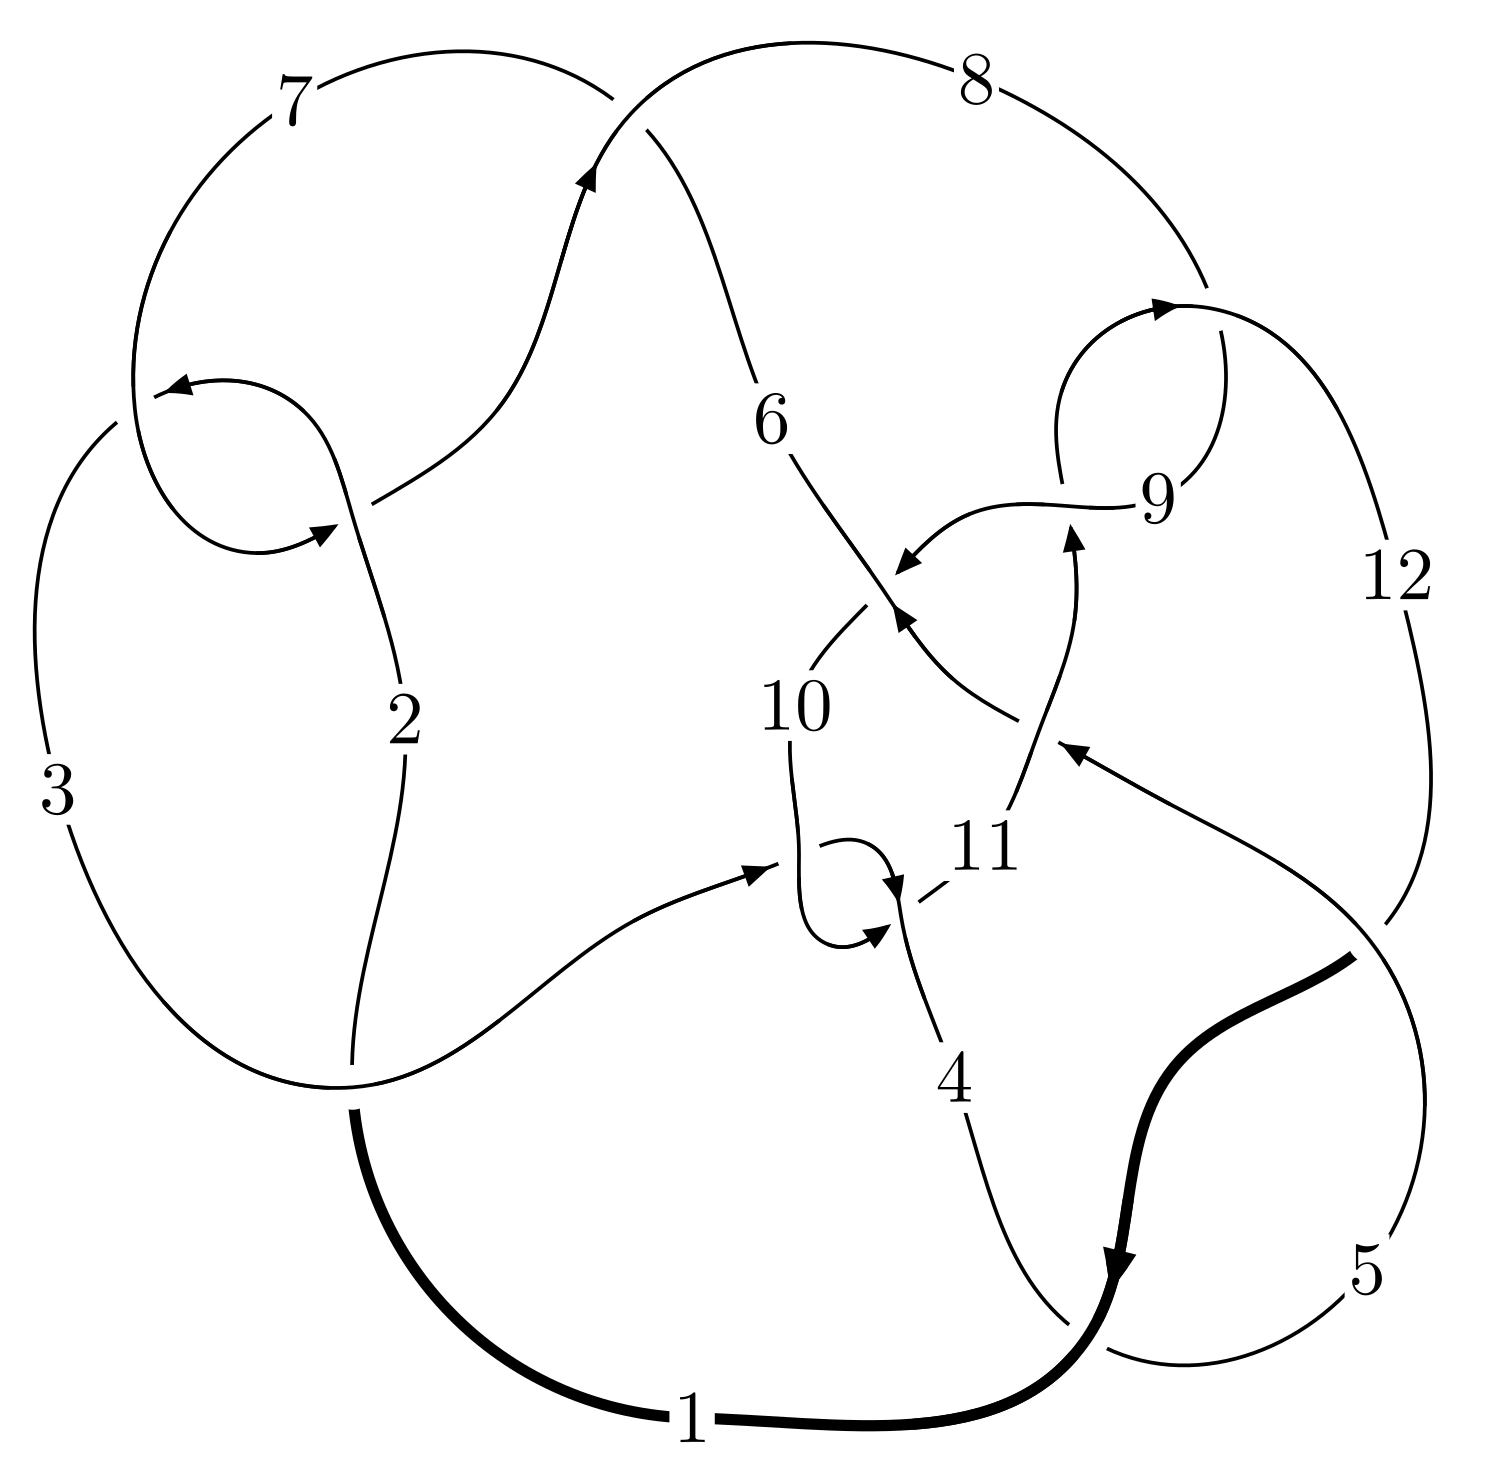
\includegraphics[width=112pt]{../../../GIT/diagram.site/Diagrams/png/1467_12a_0666.png}\\
\ \ \ A knot diagram\footnotemark}&
\allowdisplaybreaks
\textbf{Linearized knot diagam} \\
\cline{2-2}
 &
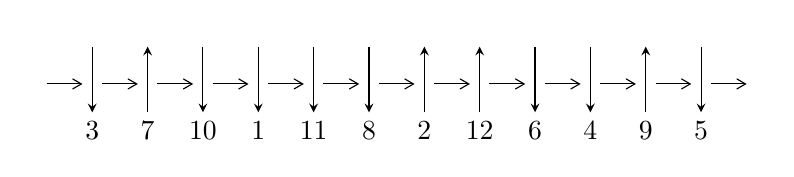
\begin{tikzpicture}[x=20pt, y=17pt]
	% nodes
	\node (C0) at (0, 0) {};
	\node (C1) at (1, 0) {};
	\node (C1U) at (1, +1) {};
	\node (C1D) at (1, -1) {3};

	\node (C2) at (2, 0) {};
	\node (C2U) at (2, +1) {};
	\node (C2D) at (2, -1) {7};

	\node (C3) at (3, 0) {};
	\node (C3U) at (3, +1) {};
	\node (C3D) at (3, -1) {10};

	\node (C4) at (4, 0) {};
	\node (C4U) at (4, +1) {};
	\node (C4D) at (4, -1) {1};

	\node (C5) at (5, 0) {};
	\node (C5U) at (5, +1) {};
	\node (C5D) at (5, -1) {11};

	\node (C6) at (6, 0) {};
	\node (C6U) at (6, +1) {};
	\node (C6D) at (6, -1) {8};

	\node (C7) at (7, 0) {};
	\node (C7U) at (7, +1) {};
	\node (C7D) at (7, -1) {2};

	\node (C8) at (8, 0) {};
	\node (C8U) at (8, +1) {};
	\node (C8D) at (8, -1) {12};

	\node (C9) at (9, 0) {};
	\node (C9U) at (9, +1) {};
	\node (C9D) at (9, -1) {6};

	\node (C10) at (10, 0) {};
	\node (C10U) at (10, +1) {};
	\node (C10D) at (10, -1) {4};

	\node (C11) at (11, 0) {};
	\node (C11U) at (11, +1) {};
	\node (C11D) at (11, -1) {9};

	\node (C12) at (12, 0) {};
	\node (C12U) at (12, +1) {};
	\node (C12D) at (12, -1) {5};
	\node (C13) at (13, 0) {};

	% arrows
	\draw[->,>={angle 60}]
	(C0) edge (C1) (C1) edge (C2) (C2) edge (C3) (C3) edge (C4) (C4) edge (C5) (C5) edge (C6) (C6) edge (C7) (C7) edge (C8) (C8) edge (C9) (C9) edge (C10) (C10) edge (C11) (C11) edge (C12) (C12) edge (C13) ;	\draw[->,>=stealth]
	(C1U) edge (C1D) (C2D) edge (C2U) (C3U) edge (C3D) (C4U) edge (C4D) (C5U) edge (C5D) (C6U) edge (C6D) (C7D) edge (C7U) (C8D) edge (C8U) (C9U) edge (C9D) (C10U) edge (C10D) (C11D) edge (C11U) (C12U) edge (C12D) ;
	\end{tikzpicture} \\
\hhline{~~} \\& 
\textbf{Solving Sequence} \\ \cline{2-2} 
 &
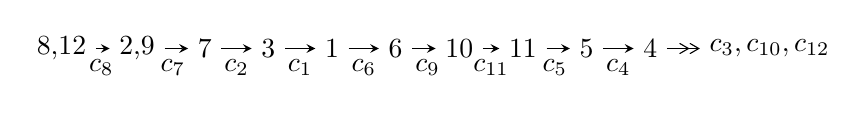
\begin{tikzpicture}[x=23pt, y=7pt]
	% node
	\node (A0) at (-1/8, 0) {8,12};
	\node (A1) at (17/16, 0) {2,9};
	\node (A2) at (17/8, 0) {7};
	\node (A3) at (25/8, 0) {3};
	\node (A4) at (33/8, 0) {1};
	\node (A5) at (41/8, 0) {6};
	\node (A6) at (49/8, 0) {10};
	\node (A7) at (57/8, 0) {11};
	\node (A8) at (65/8, 0) {5};
	\node (A9) at (73/8, 0) {4};
	\node (C1) at (1/2, -1) {$c_{8}$};
	\node (C2) at (13/8, -1) {$c_{7}$};
	\node (C3) at (21/8, -1) {$c_{2}$};
	\node (C4) at (29/8, -1) {$c_{1}$};
	\node (C5) at (37/8, -1) {$c_{6}$};
	\node (C6) at (45/8, -1) {$c_{9}$};
	\node (C7) at (53/8, -1) {$c_{11}$};
	\node (C8) at (61/8, -1) {$c_{5}$};
	\node (C9) at (69/8, -1) {$c_{4}$};
	\node (A10) at (11, 0) {$c_{3},c_{10},c_{12}$};

	% edge
	\draw[->,>=stealth]	
	(A0) edge (A1) (A1) edge (A2) (A2) edge (A3) (A3) edge (A4) (A4) edge (A5) (A5) edge (A6) (A6) edge (A7) (A7) edge (A8) (A8) edge (A9) ;
	\draw[->>,>={angle 60}]	
	(A9) edge (A10);
\end{tikzpicture} \\ 

\end{tabular} \\

\footnotetext{
The image of knot diagram is generated by the software ``\textbf{Draw programme}" developed by Andrew Bartholomew(\url{http://www.layer8.co.uk/maths/draw/index.htm\#Running-draw}), where we modified some parts for our purpose(\url{https://github.com/CATsTAILs/LinksPainter}).
}\phantom \\ \newline 
\centering \textbf{Ideals for irreducible components\footnotemark of $X_{\text{par}}$} 
 
\begin{align*}
I^u_{1}&=\langle 
-1.92536\times10^{447} u^{136}-1.57456\times10^{447} u^{135}+\cdots+2.39588\times10^{446} b+4.72928\times10^{450},\\
\phantom{I^u_{1}}&\phantom{= \langle  }-3.48036\times10^{450} u^{136}-1.65662\times10^{451} u^{135}+\cdots+3.33746\times10^{449} a-1.48601\times10^{454},\\
\phantom{I^u_{1}}&\phantom{= \langle  }u^{137}+3 u^{136}+\cdots+12298 u+1393\rangle \\
I^u_{2}&=\langle 
-37 u^{33}-194 u^{32}+\cdots+b+52,\;53 u^{33}+297 u^{32}+\cdots+a-41,\;u^{34}+6 u^{33}+\cdots+6 u+1\rangle \\
\\
\end{align*}
\raggedright * 2 irreducible components of $\dim_{\mathbb{C}}=0$, with total 171 representations.\\
\footnotetext{All coefficients of polynomials are rational numbers. But the coefficients are sometimes approximated in decimal forms when there is not enough margin.}
\newpage
\renewcommand{\arraystretch}{1}
\centering \section*{I. $I^u_{1}= \langle -1.93\times10^{447} u^{136}-1.57\times10^{447} u^{135}+\cdots+2.40\times10^{446} b+4.73\times10^{450},\;-3.48\times10^{450} u^{136}-1.66\times10^{451} u^{135}+\cdots+3.34\times10^{449} a-1.49\times10^{454},\;u^{137}+3 u^{136}+\cdots+12298 u+1393 \rangle$}
\flushleft \textbf{(i) Arc colorings}\\
\begin{tabular}{m{7pt} m{180pt} m{7pt} m{180pt} }
\flushright $a_{8}=$&$\begin{pmatrix}1\\0\end{pmatrix}$ \\
\flushright $a_{12}=$&$\begin{pmatrix}0\\u\end{pmatrix}$ \\
\flushright $a_{2}=$&$\begin{pmatrix}10.4282 u^{136}+49.6372 u^{135}+\cdots+370840. u+44525.3\\8.03614 u^{136}+6.57193 u^{135}+\cdots-142787. u-19739.2\end{pmatrix}$ \\
\flushright $a_{9}=$&$\begin{pmatrix}1\\- u^2\end{pmatrix}$ \\
\flushright $a_{7}=$&$\begin{pmatrix}-11.7845 u^{136}-76.5988 u^{135}+\cdots-698843. u-85744.5\\-14.2129 u^{136}-12.7212 u^{135}+\cdots+238819. u+33252.7\end{pmatrix}$ \\
\flushright $a_{3}=$&$\begin{pmatrix}22.0351 u^{136}+110.468 u^{135}+\cdots+864379. u+104191.\\20.1032 u^{136}+18.1880 u^{135}+\cdots-333364. u-46394.0\end{pmatrix}$ \\
\flushright $a_{1}=$&$\begin{pmatrix}-0.643174 u^{136}-15.6030 u^{135}+\cdots-187575. u-23560.4\\-0.834262 u^{136}+1.08169 u^{135}+\cdots+37569.5 u+4944.21\end{pmatrix}$ \\
\flushright $a_{6}=$&$\begin{pmatrix}-25.9974 u^{136}-89.3200 u^{135}+\cdots-460024. u-52491.8\\-14.2129 u^{136}-12.7212 u^{135}+\cdots+238819. u+33252.7\end{pmatrix}$ \\
\flushright $a_{10}=$&$\begin{pmatrix}24.9079 u^{136}+68.9754 u^{135}+\cdots+218947. u+22439.7\\-10.4660 u^{136}-39.8991 u^{135}+\cdots-237662. u-27835.2\end{pmatrix}$ \\
\flushright $a_{11}=$&$\begin{pmatrix}- u\\u^3+u\end{pmatrix}$ \\
\flushright $a_{5}=$&$\begin{pmatrix}-21.9691 u^{136}-85.4323 u^{135}+\cdots-521504. u-61150.8\\-21.1785 u^{136}-29.9099 u^{135}+\cdots+205101. u+30493.0\end{pmatrix}$ \\
\flushright $a_{4}=$&$\begin{pmatrix}13.2695 u^{136}+95.3119 u^{135}+\cdots+923969. u+113612.\\28.7003 u^{136}+42.3559 u^{135}+\cdots-266352. u-39877.1\end{pmatrix}$\\&\end{tabular}
\flushleft \textbf{(ii) Obstruction class $= -1$}\\~\\
\flushleft \textbf{(iii) Cusp Shapes $= 7.98852 u^{136}+41.2715 u^{135}+\cdots+305649. u+36865.9$}\\~\\
\newpage\renewcommand{\arraystretch}{1}
\flushleft \textbf{(iv) u-Polynomials at the component}\newline \\
\begin{tabular}{m{50pt}|m{274pt}}
Crossings & \hspace{64pt}u-Polynomials at each crossing \\
\hline $$\begin{aligned}c_{1},c_{6}\end{aligned}$$&$\begin{aligned}
&u^{137}+45 u^{136}+\cdots-444418 u-20449
\end{aligned}$\\
\hline $$\begin{aligned}c_{2},c_{7}\end{aligned}$$&$\begin{aligned}
&u^{137}+u^{136}+\cdots+702 u+143
\end{aligned}$\\
\hline $$\begin{aligned}c_{3},c_{10}\end{aligned}$$&$\begin{aligned}
&u^{137}- u^{136}+\cdots+u+1
\end{aligned}$\\
\hline $$\begin{aligned}c_{4},c_{12}\end{aligned}$$&$\begin{aligned}
&u^{137}-3 u^{136}+\cdots-6424 u+2032
\end{aligned}$\\
\hline $$\begin{aligned}c_{5}\end{aligned}$$&$\begin{aligned}
&u^{137}+u^{136}+\cdots+13177 u+477
\end{aligned}$\\
\hline $$\begin{aligned}c_{8},c_{11}\end{aligned}$$&$\begin{aligned}
&u^{137}+3 u^{136}+\cdots+12298 u+1393
\end{aligned}$\\
\hline $$\begin{aligned}c_{9}\end{aligned}$$&$\begin{aligned}
&u^{137}-3 u^{136}+\cdots+171627 u-48532
\end{aligned}$\\
\hline
\end{tabular}\\~\\
\newpage\renewcommand{\arraystretch}{1}
\flushleft \textbf{(v) Riley Polynomials at the component}\newline \\
\begin{tabular}{m{50pt}|m{274pt}}
Crossings & \hspace{64pt}Riley Polynomials at each crossing \\
\hline $$\begin{aligned}c_{1},c_{6}\end{aligned}$$&$\begin{aligned}
&y^{137}+109 y^{136}+\cdots-5228485158 y-418161601
\end{aligned}$\\
\hline $$\begin{aligned}c_{2},c_{7}\end{aligned}$$&$\begin{aligned}
&y^{137}+45 y^{136}+\cdots-444418 y-20449
\end{aligned}$\\
\hline $$\begin{aligned}c_{3},c_{10}\end{aligned}$$&$\begin{aligned}
&y^{137}-71 y^{136}+\cdots+33 y-1
\end{aligned}$\\
\hline $$\begin{aligned}c_{4},c_{12}\end{aligned}$$&$\begin{aligned}
&y^{137}+95 y^{136}+\cdots-264913984 y-4129024
\end{aligned}$\\
\hline $$\begin{aligned}c_{5}\end{aligned}$$&$\begin{aligned}
&y^{137}-9 y^{136}+\cdots+72296587 y-227529
\end{aligned}$\\
\hline $$\begin{aligned}c_{8},c_{11}\end{aligned}$$&$\begin{aligned}
&y^{137}+69 y^{136}+\cdots-92146942 y-1940449
\end{aligned}$\\
\hline $$\begin{aligned}c_{9}\end{aligned}$$&$\begin{aligned}
&y^{137}-11 y^{136}+\cdots+35394493841 y-2355355024
\end{aligned}$\\
\hline
\end{tabular}\\~\\
\newpage\flushleft \textbf{(vi) Complex Volumes and Cusp Shapes}
$$\begin{array}{c|c|c}  
\text{Solutions to }I^u_{1}& \I (\text{vol} + \sqrt{-1}CS) & \text{Cusp shape}\\
 \hline 
\begin{aligned}
u &= -0.993143 + 0.101701 I \\
a &= -0.218165 - 0.232465 I \\
b &= \phantom{-}0.215078 + 1.068600 I\end{aligned}
 & -1.65595 + 6.89184 I & \phantom{-0.000000 } 0 \\ \hline\begin{aligned}
u &= -0.993143 - 0.101701 I \\
a &= -0.218165 + 0.232465 I \\
b &= \phantom{-}0.215078 - 1.068600 I\end{aligned}
 & -1.65595 - 6.89184 I & \phantom{-0.000000 } 0 \\ \hline\begin{aligned}
u &= \phantom{-}0.392533 + 0.907153 I \\
a &= -1.54339 + 1.44894 I \\
b &= \phantom{-}0.716841 + 1.084560 I\end{aligned}
 & \phantom{-}3.05117 + 9.19531 I & \phantom{-0.000000 } 0 \\ \hline\begin{aligned}
u &= \phantom{-}0.392533 - 0.907153 I \\
a &= -1.54339 - 1.44894 I \\
b &= \phantom{-}0.716841 - 1.084560 I\end{aligned}
 & \phantom{-}3.05117 - 9.19531 I & \phantom{-0.000000 } 0 \\ \hline\begin{aligned}
u &= \phantom{-}0.335737 + 0.917551 I \\
a &= -2.64118 + 2.15957 I \\
b &= \phantom{-}0.715749 + 0.845361 I\end{aligned}
 & \phantom{-}3.44248 + 0.46124 I & \phantom{-0.000000 } 0 \\ \hline\begin{aligned}
u &= \phantom{-}0.335737 - 0.917551 I \\
a &= -2.64118 - 2.15957 I \\
b &= \phantom{-}0.715749 - 0.845361 I\end{aligned}
 & \phantom{-}3.44248 - 0.46124 I & \phantom{-0.000000 } 0 \\ \hline\begin{aligned}
u &= \phantom{-}0.419337 + 0.870394 I \\
a &= \phantom{-}0.66926 + 1.81274 I \\
b &= \phantom{-}0.709268 - 0.897251 I\end{aligned}
 & \phantom{-}3.28050 - 4.99373 I & \phantom{-0.000000 } 0 \\ \hline\begin{aligned}
u &= \phantom{-}0.419337 - 0.870394 I \\
a &= \phantom{-}0.66926 - 1.81274 I \\
b &= \phantom{-}0.709268 + 0.897251 I\end{aligned}
 & \phantom{-}3.28050 + 4.99373 I & \phantom{-0.000000 } 0 \\ \hline\begin{aligned}
u &= -0.516989 + 0.804672 I \\
a &= -0.579232 + 0.152322 I \\
b &= -0.229961 + 0.657869 I\end{aligned}
 & -5.23773 - 2.94305 I & \phantom{-0.000000 } 0 \\ \hline\begin{aligned}
u &= -0.516989 - 0.804672 I \\
a &= -0.579232 - 0.152322 I \\
b &= -0.229961 - 0.657869 I\end{aligned}
 & -5.23773 + 2.94305 I & \phantom{-0.000000 } 0\\
 \hline 
 \end{array}$$\newpage$$\begin{array}{c|c|c}  
\text{Solutions to }I^u_{1}& \I (\text{vol} + \sqrt{-1}CS) & \text{Cusp shape}\\
 \hline 
\begin{aligned}
u &= -0.368298 + 0.881432 I \\
a &= \phantom{-}2.26249 + 1.16568 I \\
b &= -0.804910 + 0.958572 I\end{aligned}
 & \phantom{-}6.25192 - 4.89483 I & \phantom{-0.000000 } 0 \\ \hline\begin{aligned}
u &= -0.368298 - 0.881432 I \\
a &= \phantom{-}2.26249 - 1.16568 I \\
b &= -0.804910 - 0.958572 I\end{aligned}
 & \phantom{-}6.25192 + 4.89483 I & \phantom{-0.000000 } 0 \\ \hline\begin{aligned}
u &= -0.396093 + 0.835282 I \\
a &= \phantom{-}1.86286 + 0.16204 I \\
b &= -0.900967 + 0.906827 I\end{aligned}
 & \phantom{-}6.63966 - 4.81464 I & \phantom{-0.000000 } 0 \\ \hline\begin{aligned}
u &= -0.396093 - 0.835282 I \\
a &= \phantom{-}1.86286 - 0.16204 I \\
b &= -0.900967 - 0.906827 I\end{aligned}
 & \phantom{-}6.63966 + 4.81464 I & \phantom{-0.000000 } 0 \\ \hline\begin{aligned}
u &= -0.214491 + 1.057340 I \\
a &= \phantom{-}0.50406 - 1.35552 I \\
b &= -0.449252 - 1.022370 I\end{aligned}
 & -7.08230 + 0.25351 I & \phantom{-0.000000 } 0 \\ \hline\begin{aligned}
u &= -0.214491 - 1.057340 I \\
a &= \phantom{-}0.50406 + 1.35552 I \\
b &= -0.449252 + 1.022370 I\end{aligned}
 & -7.08230 - 0.25351 I & \phantom{-0.000000 } 0 \\ \hline\begin{aligned}
u &= \phantom{-}0.460709 + 0.795289 I \\
a &= \phantom{-}0.298432 + 0.730500 I \\
b &= \phantom{-}0.857184 - 0.587518 I\end{aligned}
 & \phantom{-}4.54617 + 3.31372 I & \phantom{-0.000000 } 0 \\ \hline\begin{aligned}
u &= \phantom{-}0.460709 - 0.795289 I \\
a &= \phantom{-}0.298432 - 0.730500 I \\
b &= \phantom{-}0.857184 + 0.587518 I\end{aligned}
 & \phantom{-}4.54617 - 3.31372 I & \phantom{-0.000000 } 0 \\ \hline\begin{aligned}
u &= \phantom{-}0.422657 + 0.813674 I \\
a &= -1.171570 - 0.202241 I \\
b &= \phantom{-}0.914540 + 0.738281 I\end{aligned}
 & \phantom{-}4.52281 + 0.41179 I & \phantom{-0.000000 } 0 \\ \hline\begin{aligned}
u &= \phantom{-}0.422657 - 0.813674 I \\
a &= -1.171570 + 0.202241 I \\
b &= \phantom{-}0.914540 - 0.738281 I\end{aligned}
 & \phantom{-}4.52281 - 0.41179 I & \phantom{-0.000000 } 0\\
 \hline 
 \end{array}$$\newpage$$\begin{array}{c|c|c}  
\text{Solutions to }I^u_{1}& \I (\text{vol} + \sqrt{-1}CS) & \text{Cusp shape}\\
 \hline 
\begin{aligned}
u &= -0.361692 + 0.841302 I \\
a &= \phantom{-}2.58809 + 0.33776 I \\
b &= -0.857062 + 0.927377 I\end{aligned}
 & \phantom{-}6.46165 - 4.79464 I & \phantom{-0.000000 } 0 \\ \hline\begin{aligned}
u &= -0.361692 - 0.841302 I \\
a &= \phantom{-}2.58809 - 0.33776 I \\
b &= -0.857062 - 0.927377 I\end{aligned}
 & \phantom{-}6.46165 + 4.79464 I & \phantom{-0.000000 } 0 \\ \hline\begin{aligned}
u &= \phantom{-}0.903691 + 0.088826 I \\
a &= \phantom{-}1.44805 + 0.24406 I \\
b &= -0.717408 - 0.832415 I\end{aligned}
 & \phantom{-}3.83282 + 2.56162 I & \phantom{-0.000000 } 0 \\ \hline\begin{aligned}
u &= \phantom{-}0.903691 - 0.088826 I \\
a &= \phantom{-}1.44805 - 0.24406 I \\
b &= -0.717408 + 0.832415 I\end{aligned}
 & \phantom{-}3.83282 - 2.56162 I & \phantom{-0.000000 } 0 \\ \hline\begin{aligned}
u &= -0.418033 + 0.804706 I \\
a &= -0.008821 + 1.147750 I \\
b &= -0.877861 - 0.810105 I\end{aligned}
 & \phantom{-}6.71587 + 1.32958 I & \phantom{-0.000000 } 0 \\ \hline\begin{aligned}
u &= -0.418033 - 0.804706 I \\
a &= -0.008821 - 1.147750 I \\
b &= -0.877861 + 0.810105 I\end{aligned}
 & \phantom{-}6.71587 - 1.32958 I & \phantom{-0.000000 } 0 \\ \hline\begin{aligned}
u &= -0.113520 + 1.087530 I \\
a &= -1.31438 - 0.79719 I \\
b &= \phantom{-}0.527247 - 0.883145 I\end{aligned}
 & -1.72816 - 2.72038 I & \phantom{-0.000000 } 0 \\ \hline\begin{aligned}
u &= -0.113520 - 1.087530 I \\
a &= -1.31438 + 0.79719 I \\
b &= \phantom{-}0.527247 + 0.883145 I\end{aligned}
 & -1.72816 + 2.72038 I & \phantom{-0.000000 } 0 \\ \hline\begin{aligned}
u &= \phantom{-}0.896144 + 0.070680 I \\
a &= \phantom{-}1.176020 + 0.576398 I \\
b &= -0.702580 - 0.907849 I\end{aligned}
 & \phantom{-}3.60119 + 2.87209 I & \phantom{-0.000000 } 0 \\ \hline\begin{aligned}
u &= \phantom{-}0.896144 - 0.070680 I \\
a &= \phantom{-}1.176020 - 0.576398 I \\
b &= -0.702580 + 0.907849 I\end{aligned}
 & \phantom{-}3.60119 - 2.87209 I & \phantom{-0.000000 } 0\\
 \hline 
 \end{array}$$\newpage$$\begin{array}{c|c|c}  
\text{Solutions to }I^u_{1}& \I (\text{vol} + \sqrt{-1}CS) & \text{Cusp shape}\\
 \hline 
\begin{aligned}
u &= -0.367760 + 0.813349 I \\
a &= \phantom{-}0.60666 + 1.64872 I \\
b &= -0.862981 - 0.900064 I\end{aligned}
 & \phantom{-}6.54515 + 1.58431 I & \phantom{-0.000000 } 0 \\ \hline\begin{aligned}
u &= -0.367760 - 0.813349 I \\
a &= \phantom{-}0.60666 - 1.64872 I \\
b &= -0.862981 + 0.900064 I\end{aligned}
 & \phantom{-}6.54515 - 1.58431 I & \phantom{-0.000000 } 0 \\ \hline\begin{aligned}
u &= \phantom{-}0.451707 + 1.019320 I \\
a &= \phantom{-}1.60939 + 0.51494 I \\
b &= -0.173522 - 0.796738 I\end{aligned}
 & -2.15556 + 5.13134 I & \phantom{-0.000000 } 0 \\ \hline\begin{aligned}
u &= \phantom{-}0.451707 - 1.019320 I \\
a &= \phantom{-}1.60939 - 0.51494 I \\
b &= -0.173522 + 0.796738 I\end{aligned}
 & -2.15556 - 5.13134 I & \phantom{-0.000000 } 0 \\ \hline\begin{aligned}
u &= \phantom{-}0.804434 + 0.334261 I \\
a &= \phantom{-}0.976121 - 0.598655 I \\
b &= -0.444550 - 0.275846 I\end{aligned}
 & \phantom{-}3.40481 + 1.01507 I & \phantom{-0.000000 } 0 \\ \hline\begin{aligned}
u &= \phantom{-}0.804434 - 0.334261 I \\
a &= \phantom{-}0.976121 + 0.598655 I \\
b &= -0.444550 + 0.275846 I\end{aligned}
 & \phantom{-}3.40481 - 1.01507 I & \phantom{-0.000000 } 0 \\ \hline\begin{aligned}
u &= -1.072280 + 0.366077 I \\
a &= \phantom{-}1.63883 - 0.56764 I \\
b &= -0.860414 + 0.716196 I\end{aligned}
 & \phantom{-}5.54552 + 6.60550 I & \phantom{-0.000000 } 0 \\ \hline\begin{aligned}
u &= -1.072280 - 0.366077 I \\
a &= \phantom{-}1.63883 + 0.56764 I \\
b &= -0.860414 - 0.716196 I\end{aligned}
 & \phantom{-}5.54552 - 6.60550 I & \phantom{-0.000000 } 0 \\ \hline\begin{aligned}
u &= \phantom{-}0.327386 + 1.085800 I \\
a &= \phantom{-}0.049409 + 0.759822 I \\
b &= -0.165832 + 1.204450 I\end{aligned}
 & -3.49765 + 0.87772 I & \phantom{-0.000000 } 0 \\ \hline\begin{aligned}
u &= \phantom{-}0.327386 - 1.085800 I \\
a &= \phantom{-}0.049409 - 0.759822 I \\
b &= -0.165832 - 1.204450 I\end{aligned}
 & -3.49765 - 0.87772 I & \phantom{-0.000000 } 0\\
 \hline 
 \end{array}$$\newpage$$\begin{array}{c|c|c}  
\text{Solutions to }I^u_{1}& \I (\text{vol} + \sqrt{-1}CS) & \text{Cusp shape}\\
 \hline 
\begin{aligned}
u &= \phantom{-}0.164764 + 0.848550 I \\
a &= -0.326735 - 0.251444 I \\
b &= \phantom{-}0.508569 + 0.345209 I\end{aligned}
 & -0.392647 + 1.151400 I & \phantom{-0.000000 } 0 \\ \hline\begin{aligned}
u &= \phantom{-}0.164764 - 0.848550 I \\
a &= -0.326735 + 0.251444 I \\
b &= \phantom{-}0.508569 - 0.345209 I\end{aligned}
 & -0.392647 - 1.151400 I & \phantom{-0.000000 } 0 \\ \hline\begin{aligned}
u &= -0.400949 + 1.064290 I \\
a &= -0.698332 - 0.958258 I \\
b &= \phantom{-}0.720921 + 0.502062 I\end{aligned}
 & -1.42672 + 0.77872 I & \phantom{-0.000000 } 0 \\ \hline\begin{aligned}
u &= -0.400949 - 1.064290 I \\
a &= -0.698332 + 0.958258 I \\
b &= \phantom{-}0.720921 - 0.502062 I\end{aligned}
 & -1.42672 - 0.77872 I & \phantom{-0.000000 } 0 \\ \hline\begin{aligned}
u &= -0.364467 + 0.780883 I \\
a &= \phantom{-}0.878470 + 1.096230 I \\
b &= -0.866933 - 0.921688 I\end{aligned}
 & \phantom{-}6.57472 + 1.68871 I & \phantom{-0.000000 } 0 \\ \hline\begin{aligned}
u &= -0.364467 - 0.780883 I \\
a &= \phantom{-}0.878470 - 1.096230 I \\
b &= -0.866933 + 0.921688 I\end{aligned}
 & \phantom{-}6.57472 - 1.68871 I & \phantom{-0.000000 } 0 \\ \hline\begin{aligned}
u &= \phantom{-}0.367939 + 0.777842 I \\
a &= -2.49524 - 1.09866 I \\
b &= \phantom{-}0.782216 + 0.937556 I\end{aligned}
 & \phantom{-}3.62022 + 8.40450 I & \phantom{-0.000000 } 0 \\ \hline\begin{aligned}
u &= \phantom{-}0.367939 - 0.777842 I \\
a &= -2.49524 + 1.09866 I \\
b &= \phantom{-}0.782216 - 0.937556 I\end{aligned}
 & \phantom{-}3.62022 - 8.40450 I & \phantom{-0.000000 } 0 \\ \hline\begin{aligned}
u &= -0.384630 + 1.077120 I \\
a &= \phantom{-}0.196232 + 0.403779 I \\
b &= -0.594972 + 0.100972 I\end{aligned}
 & -4.76593 - 3.47175 I & \phantom{-0.000000 } 0 \\ \hline\begin{aligned}
u &= -0.384630 - 1.077120 I \\
a &= \phantom{-}0.196232 - 0.403779 I \\
b &= -0.594972 - 0.100972 I\end{aligned}
 & -4.76593 + 3.47175 I & \phantom{-0.000000 } 0\\
 \hline 
 \end{array}$$\newpage$$\begin{array}{c|c|c}  
\text{Solutions to }I^u_{1}& \I (\text{vol} + \sqrt{-1}CS) & \text{Cusp shape}\\
 \hline 
\begin{aligned}
u &= \phantom{-}0.304451 + 0.778083 I \\
a &= -2.15880 + 1.44622 I \\
b &= \phantom{-}0.816538 - 0.837720 I\end{aligned}
 & \phantom{-}3.93353 + 2.41327 I & \phantom{-0.000000 } 0 \\ \hline\begin{aligned}
u &= \phantom{-}0.304451 - 0.778083 I \\
a &= -2.15880 - 1.44622 I \\
b &= \phantom{-}0.816538 + 0.837720 I\end{aligned}
 & \phantom{-}3.93353 - 2.41327 I & \phantom{-0.000000 } 0 \\ \hline\begin{aligned}
u &= -0.828620 + 0.007884 I \\
a &= -1.85148 - 0.35762 I \\
b &= \phantom{-}0.759856 + 0.964455 I\end{aligned}
 & \phantom{-}1.39093 + 7.00393 I & \phantom{-0.000000 } 0 \\ \hline\begin{aligned}
u &= -0.828620 - 0.007884 I \\
a &= -1.85148 + 0.35762 I \\
b &= \phantom{-}0.759856 - 0.964455 I\end{aligned}
 & \phantom{-}1.39093 - 7.00393 I & \phantom{-0.000000 } 0 \\ \hline\begin{aligned}
u &= \phantom{-}0.014036 + 0.825161 I \\
a &= -1.43561 - 4.31284 I \\
b &= \phantom{-}0.129023 - 0.728985 I\end{aligned}
 & \phantom{-}0.28990 - 2.20949 I & \phantom{-0.000000 } 0 \\ \hline\begin{aligned}
u &= \phantom{-}0.014036 - 0.825161 I \\
a &= -1.43561 + 4.31284 I \\
b &= \phantom{-}0.129023 + 0.728985 I\end{aligned}
 & \phantom{-}0.28990 + 2.20949 I & \phantom{-0.000000 } 0 \\ \hline\begin{aligned}
u &= \phantom{-}0.355556 + 0.742629 I \\
a &= -1.026380 + 0.177768 I \\
b &= \phantom{-}0.801561 - 1.032050 I\end{aligned}
 & \phantom{-}3.61646 - 5.91274 I & \phantom{-0.000000 } 0 \\ \hline\begin{aligned}
u &= \phantom{-}0.355556 - 0.742629 I \\
a &= -1.026380 - 0.177768 I \\
b &= \phantom{-}0.801561 + 1.032050 I\end{aligned}
 & \phantom{-}3.61646 + 5.91274 I & \phantom{-0.000000 } 0 \\ \hline\begin{aligned}
u &= -1.139030 + 0.338886 I \\
a &= \phantom{-}1.55291 + 0.58164 I \\
b &= -0.754410 - 1.020510 I\end{aligned}
 & \phantom{-}4.60598 + 12.61970 I & \phantom{-0.000000 } 0 \\ \hline\begin{aligned}
u &= -1.139030 - 0.338886 I \\
a &= \phantom{-}1.55291 - 0.58164 I \\
b &= -0.754410 + 1.020510 I\end{aligned}
 & \phantom{-}4.60598 - 12.61970 I & \phantom{-0.000000 } 0\\
 \hline 
 \end{array}$$\newpage$$\begin{array}{c|c|c}  
\text{Solutions to }I^u_{1}& \I (\text{vol} + \sqrt{-1}CS) & \text{Cusp shape}\\
 \hline 
\begin{aligned}
u &= -0.375911 + 1.135100 I \\
a &= -0.142324 + 0.445881 I \\
b &= \phantom{-}0.413396 + 1.237030 I\end{aligned}
 & -4.31323 - 3.59247 I & \phantom{-0.000000 } 0 \\ \hline\begin{aligned}
u &= -0.375911 - 1.135100 I \\
a &= -0.142324 - 0.445881 I \\
b &= \phantom{-}0.413396 - 1.237030 I\end{aligned}
 & -4.31323 + 3.59247 I & \phantom{-0.000000 } 0 \\ \hline\begin{aligned}
u &= -0.363577 + 1.159620 I \\
a &= -1.220750 - 0.367940 I \\
b &= \phantom{-}0.669024 - 0.724481 I\end{aligned}
 & -1.91888 - 2.86850 I & \phantom{-0.000000 } 0 \\ \hline\begin{aligned}
u &= -0.363577 - 1.159620 I \\
a &= -1.220750 + 0.367940 I \\
b &= \phantom{-}0.669024 + 0.724481 I\end{aligned}
 & -1.91888 + 2.86850 I & \phantom{-0.000000 } 0 \\ \hline\begin{aligned}
u &= -0.778000 + 0.066848 I \\
a &= -1.42799 + 0.91687 I \\
b &= \phantom{-}0.810378 - 0.785210 I\end{aligned}
 & \phantom{-}1.94160 + 1.10807 I & \phantom{-0.000000 } 0 \\ \hline\begin{aligned}
u &= -0.778000 - 0.066848 I \\
a &= -1.42799 - 0.91687 I \\
b &= \phantom{-}0.810378 + 0.785210 I\end{aligned}
 & \phantom{-}1.94160 - 1.10807 I & \phantom{-0.000000 } 0 \\ \hline\begin{aligned}
u &= \phantom{-}0.264817 + 1.196190 I \\
a &= -0.294259 + 1.340730 I \\
b &= \phantom{-}0.063453 + 0.987721 I\end{aligned}
 & -4.34457 + 2.46575 I & \phantom{-0.000000 } 0 \\ \hline\begin{aligned}
u &= \phantom{-}0.264817 - 1.196190 I \\
a &= -0.294259 - 1.340730 I \\
b &= \phantom{-}0.063453 - 0.987721 I\end{aligned}
 & -4.34457 - 2.46575 I & \phantom{-0.000000 } 0 \\ \hline\begin{aligned}
u &= \phantom{-}0.162186 + 1.222950 I \\
a &= \phantom{-}1.163560 + 0.247869 I \\
b &= -0.473152 + 0.605479 I\end{aligned}
 & -1.49506 + 2.98930 I & \phantom{-0.000000 } 0 \\ \hline\begin{aligned}
u &= \phantom{-}0.162186 - 1.222950 I \\
a &= \phantom{-}1.163560 - 0.247869 I \\
b &= -0.473152 - 0.605479 I\end{aligned}
 & -1.49506 - 2.98930 I & \phantom{-0.000000 } 0\\
 \hline 
 \end{array}$$\newpage$$\begin{array}{c|c|c}  
\text{Solutions to }I^u_{1}& \I (\text{vol} + \sqrt{-1}CS) & \text{Cusp shape}\\
 \hline 
\begin{aligned}
u &= \phantom{-}0.522387 + 1.125440 I \\
a &= \phantom{-}0.635698 - 0.248411 I \\
b &= -0.717731 + 0.117324 I\end{aligned}
 & \phantom{-}0.98211 + 3.85776 I & \phantom{-0.000000 } 0 \\ \hline\begin{aligned}
u &= \phantom{-}0.522387 - 1.125440 I \\
a &= \phantom{-}0.635698 + 0.248411 I \\
b &= -0.717731 - 0.117324 I\end{aligned}
 & \phantom{-}0.98211 - 3.85776 I & \phantom{-0.000000 } 0 \\ \hline\begin{aligned}
u &= -0.360988 + 1.188570 I \\
a &= \phantom{-}0.95877 + 1.46767 I \\
b &= -0.210270 + 1.053090 I\end{aligned}
 & -8.38401 - 6.17019 I & \phantom{-0.000000 } 0 \\ \hline\begin{aligned}
u &= -0.360988 - 1.188570 I \\
a &= \phantom{-}0.95877 - 1.46767 I \\
b &= -0.210270 - 1.053090 I\end{aligned}
 & -8.38401 + 6.17019 I & \phantom{-0.000000 } 0 \\ \hline\begin{aligned}
u &= -0.498190 + 1.145610 I \\
a &= -0.784141 - 0.350457 I \\
b &= \phantom{-}0.922097 - 0.125766 I\end{aligned}
 & -0.64331 - 8.43493 I & \phantom{-0.000000 } 0 \\ \hline\begin{aligned}
u &= -0.498190 - 1.145610 I \\
a &= -0.784141 + 0.350457 I \\
b &= \phantom{-}0.922097 + 0.125766 I\end{aligned}
 & -0.64331 + 8.43493 I & \phantom{-0.000000 } 0 \\ \hline\begin{aligned}
u &= \phantom{-}0.555101 + 1.139340 I \\
a &= \phantom{-}0.429042 - 0.506563 I \\
b &= -0.716737 + 0.615005 I\end{aligned}
 & \phantom{-}0.83561 + 2.66881 I & \phantom{-0.000000 } 0 \\ \hline\begin{aligned}
u &= \phantom{-}0.555101 - 1.139340 I \\
a &= \phantom{-}0.429042 + 0.506563 I \\
b &= -0.716737 - 0.615005 I\end{aligned}
 & \phantom{-}0.83561 - 2.66881 I & \phantom{-0.000000 } 0 \\ \hline\begin{aligned}
u &= -0.699115 + 0.214848 I \\
a &= -1.20389 - 0.93781 I \\
b &= \phantom{-}0.707081 + 0.058289 I\end{aligned}
 & \phantom{-}2.06768 + 3.88854 I & \phantom{-0.000000 } 0 \\ \hline\begin{aligned}
u &= -0.699115 - 0.214848 I \\
a &= -1.20389 + 0.93781 I \\
b &= \phantom{-}0.707081 - 0.058289 I\end{aligned}
 & \phantom{-}2.06768 - 3.88854 I & \phantom{-0.000000 } 0\\
 \hline 
 \end{array}$$\newpage$$\begin{array}{c|c|c}  
\text{Solutions to }I^u_{1}& \I (\text{vol} + \sqrt{-1}CS) & \text{Cusp shape}\\
 \hline 
\begin{aligned}
u &= -0.476043 + 1.180790 I \\
a &= -0.102158 - 0.957535 I \\
b &= \phantom{-}0.851883 + 0.737158 I\end{aligned}
 & -1.28877 - 5.63444 I & \phantom{-0.000000 } 0 \\ \hline\begin{aligned}
u &= -0.476043 - 1.180790 I \\
a &= -0.102158 + 0.957535 I \\
b &= \phantom{-}0.851883 - 0.737158 I\end{aligned}
 & -1.28877 + 5.63444 I & \phantom{-0.000000 } 0 \\ \hline\begin{aligned}
u &= \phantom{-}1.251420 + 0.281998 I \\
a &= \phantom{-}0.276455 + 0.147205 I \\
b &= -0.140848 + 0.858327 I\end{aligned}
 & \phantom{-}1.76672 - 1.02889 I & \phantom{-0.000000 } 0 \\ \hline\begin{aligned}
u &= \phantom{-}1.251420 - 0.281998 I \\
a &= \phantom{-}0.276455 - 0.147205 I \\
b &= -0.140848 - 0.858327 I\end{aligned}
 & \phantom{-}1.76672 + 1.02889 I & \phantom{-0.000000 } 0 \\ \hline\begin{aligned}
u &= -0.579676 + 1.154700 I \\
a &= -1.93844 - 0.37344 I \\
b &= \phantom{-}0.622082 - 1.026640 I\end{aligned}
 & -2.92632 - 4.30812 I & \phantom{-0.000000 } 0 \\ \hline\begin{aligned}
u &= -0.579676 - 1.154700 I \\
a &= -1.93844 + 0.37344 I \\
b &= \phantom{-}0.622082 + 1.026640 I\end{aligned}
 & -2.92632 + 4.30812 I & \phantom{-0.000000 } 0 \\ \hline\begin{aligned}
u &= -0.856923 + 0.968536 I \\
a &= \phantom{-}1.23974 + 1.20572 I \\
b &= -0.711815 - 0.829718 I\end{aligned}
 & -2.50811 - 0.59518 I & \phantom{-0.000000 } 0 \\ \hline\begin{aligned}
u &= -0.856923 - 0.968536 I \\
a &= \phantom{-}1.23974 - 1.20572 I \\
b &= -0.711815 + 0.829718 I\end{aligned}
 & -2.50811 + 0.59518 I & \phantom{-0.000000 } 0 \\ \hline\begin{aligned}
u &= \phantom{-}0.088978 + 1.290330 I \\
a &= \phantom{-}0.999566 + 0.163151 I \\
b &= -0.594033 + 0.601718 I\end{aligned}
 & -1.50031 + 2.99831 I & \phantom{-0.000000 } 0 \\ \hline\begin{aligned}
u &= \phantom{-}0.088978 - 1.290330 I \\
a &= \phantom{-}0.999566 - 0.163151 I \\
b &= -0.594033 - 0.601718 I\end{aligned}
 & -1.50031 - 2.99831 I & \phantom{-0.000000 } 0\\
 \hline 
 \end{array}$$\newpage$$\begin{array}{c|c|c}  
\text{Solutions to }I^u_{1}& \I (\text{vol} + \sqrt{-1}CS) & \text{Cusp shape}\\
 \hline 
\begin{aligned}
u &= -0.477721 + 1.213540 I \\
a &= -1.96698 - 1.02776 I \\
b &= \phantom{-}0.760111 - 1.009490 I\end{aligned}
 & -2.13051 - 11.64950 I & \phantom{-0.000000 } 0 \\ \hline\begin{aligned}
u &= -0.477721 - 1.213540 I \\
a &= -1.96698 + 1.02776 I \\
b &= \phantom{-}0.760111 + 1.009490 I\end{aligned}
 & -2.13051 + 11.64950 I & \phantom{-0.000000 } 0 \\ \hline\begin{aligned}
u &= \phantom{-}0.524657 + 1.202000 I \\
a &= -0.020882 - 0.610337 I \\
b &= -0.684439 + 0.810813 I\end{aligned}
 & \phantom{-}0.28445 + 2.16636 I & \phantom{-0.000000 } 0 \\ \hline\begin{aligned}
u &= \phantom{-}0.524657 - 1.202000 I \\
a &= -0.020882 + 0.610337 I \\
b &= -0.684439 - 0.810813 I\end{aligned}
 & \phantom{-}0.28445 - 2.16636 I & \phantom{-0.000000 } 0 \\ \hline\begin{aligned}
u &= \phantom{-}1.181100 + 0.583727 I \\
a &= -1.75285 - 0.51367 I \\
b &= \phantom{-}0.793700 + 0.794483 I\end{aligned}
 & \phantom{-}7.65989 + 0.80808 I & \phantom{-0.000000 } 0 \\ \hline\begin{aligned}
u &= \phantom{-}1.181100 - 0.583727 I \\
a &= -1.75285 + 0.51367 I \\
b &= \phantom{-}0.793700 - 0.794483 I\end{aligned}
 & \phantom{-}7.65989 - 0.80808 I & \phantom{-0.000000 } 0 \\ \hline\begin{aligned}
u &= -0.637475 + 1.154780 I \\
a &= -0.908847 - 0.872106 I \\
b &= -0.023503 - 0.890496 I\end{aligned}
 & -6.63194 - 2.04469 I & \phantom{-0.000000 } 0 \\ \hline\begin{aligned}
u &= -0.637475 - 1.154780 I \\
a &= -0.908847 + 0.872106 I \\
b &= -0.023503 + 0.890496 I\end{aligned}
 & -6.63194 + 2.04469 I & \phantom{-0.000000 } 0 \\ \hline\begin{aligned}
u &= \phantom{-}0.056983 + 0.678074 I \\
a &= -0.06769 - 2.21669 I \\
b &= \phantom{-}0.109985 - 1.246770 I\end{aligned}
 & -1.54146 + 1.35035 I & \phantom{-0.000000 } 0 \\ \hline\begin{aligned}
u &= \phantom{-}0.056983 - 0.678074 I \\
a &= -0.06769 + 2.21669 I \\
b &= \phantom{-}0.109985 + 1.246770 I\end{aligned}
 & -1.54146 - 1.35035 I & \phantom{-0.000000 } 0\\
 \hline 
 \end{array}$$\newpage$$\begin{array}{c|c|c}  
\text{Solutions to }I^u_{1}& \I (\text{vol} + \sqrt{-1}CS) & \text{Cusp shape}\\
 \hline 
\begin{aligned}
u &= -0.585908 + 0.342572 I \\
a &= -1.50703 - 1.52512 I \\
b &= \phantom{-}0.372092 + 0.951869 I\end{aligned}
 & -0.770443 - 0.547292 I & \phantom{-0.000000 } 0 \\ \hline\begin{aligned}
u &= -0.585908 - 0.342572 I \\
a &= -1.50703 + 1.52512 I \\
b &= \phantom{-}0.372092 - 0.951869 I\end{aligned}
 & -0.770443 + 0.547292 I & \phantom{-0.000000 } 0 \\ \hline\begin{aligned}
u &= -0.422000 + 1.272690 I \\
a &= -0.575533 + 0.086946 I \\
b &= \phantom{-}0.679722 + 0.934991 I\end{aligned}
 & -2.49125 + 2.35660 I & \phantom{-0.000000 } 0 \\ \hline\begin{aligned}
u &= -0.422000 - 1.272690 I \\
a &= -0.575533 - 0.086946 I \\
b &= \phantom{-}0.679722 - 0.934991 I\end{aligned}
 & -2.49125 - 2.35660 I & \phantom{-0.000000 } 0 \\ \hline\begin{aligned}
u &= \phantom{-}0.487366 + 1.254290 I \\
a &= \phantom{-}1.62217 - 1.02987 I \\
b &= -0.682957 - 0.934186 I\end{aligned}
 & -0.11114 + 7.44318 I & \phantom{-0.000000 } 0 \\ \hline\begin{aligned}
u &= \phantom{-}0.487366 - 1.254290 I \\
a &= \phantom{-}1.62217 + 1.02987 I \\
b &= -0.682957 + 0.934186 I\end{aligned}
 & -0.11114 - 7.44318 I & \phantom{-0.000000 } 0 \\ \hline\begin{aligned}
u &= -0.852581 + 1.049770 I \\
a &= \phantom{-}2.30661 - 0.02185 I \\
b &= -0.704234 + 0.908771 I\end{aligned}
 & -2.75425 - 6.02344 I & \phantom{-0.000000 } 0 \\ \hline\begin{aligned}
u &= -0.852581 - 1.049770 I \\
a &= \phantom{-}2.30661 + 0.02185 I \\
b &= -0.704234 - 0.908771 I\end{aligned}
 & -2.75425 + 6.02344 I & \phantom{-0.000000 } 0 \\ \hline\begin{aligned}
u &= -0.533149 + 1.254590 I \\
a &= -1.009580 - 0.757415 I \\
b &= \phantom{-}0.249405 - 1.188060 I\end{aligned}
 & -5.21066 - 12.26540 I & \phantom{-0.000000 } 0 \\ \hline\begin{aligned}
u &= -0.533149 - 1.254590 I \\
a &= -1.009580 + 0.757415 I \\
b &= \phantom{-}0.249405 + 1.188060 I\end{aligned}
 & -5.21066 + 12.26540 I & \phantom{-0.000000 } 0\\
 \hline 
 \end{array}$$\newpage$$\begin{array}{c|c|c}  
\text{Solutions to }I^u_{1}& \I (\text{vol} + \sqrt{-1}CS) & \text{Cusp shape}\\
 \hline 
\begin{aligned}
u &= \phantom{-}1.246560 + 0.557148 I \\
a &= -1.50904 + 0.64457 I \\
b &= \phantom{-}0.749899 - 0.952042 I\end{aligned}
 & \phantom{-}7.17363 - 5.00606 I & \phantom{-0.000000 } 0 \\ \hline\begin{aligned}
u &= \phantom{-}1.246560 - 0.557148 I \\
a &= -1.50904 - 0.64457 I \\
b &= \phantom{-}0.749899 + 0.952042 I\end{aligned}
 & \phantom{-}7.17363 + 5.00606 I & \phantom{-0.000000 } 0 \\ \hline\begin{aligned}
u &= \phantom{-}0.520321 + 1.275230 I \\
a &= \phantom{-}1.42291 - 0.70314 I \\
b &= -0.646359 - 1.031850 I\end{aligned}
 & -0.41612 + 7.92072 I & \phantom{-0.000000 } 0 \\ \hline\begin{aligned}
u &= \phantom{-}0.520321 - 1.275230 I \\
a &= \phantom{-}1.42291 + 0.70314 I \\
b &= -0.646359 + 1.031850 I\end{aligned}
 & -0.41612 - 7.92072 I & \phantom{-0.000000 } 0 \\ \hline\begin{aligned}
u &= \phantom{-}0.446314 + 0.431505 I \\
a &= \phantom{-}0.28919 - 2.37502 I \\
b &= \phantom{-}0.040024 + 0.878173 I\end{aligned}
 & -0.481966 - 1.247710 I & \phantom{-0.000000 } 0 \\ \hline\begin{aligned}
u &= \phantom{-}0.446314 - 0.431505 I \\
a &= \phantom{-}0.28919 + 2.37502 I \\
b &= \phantom{-}0.040024 - 0.878173 I\end{aligned}
 & -0.481966 + 1.247710 I & \phantom{-0.000000 } 0 \\ \hline\begin{aligned}
u &= -0.653847 + 1.226990 I \\
a &= \phantom{-}0.539138 + 0.976902 I \\
b &= -0.923455 - 0.692051 I\end{aligned}
 & \phantom{-}2.81024 - 12.76900 I & \phantom{-0.000000 } 0 \\ \hline\begin{aligned}
u &= -0.653847 - 1.226990 I \\
a &= \phantom{-}0.539138 - 0.976902 I \\
b &= -0.923455 + 0.692051 I\end{aligned}
 & \phantom{-}2.81024 + 12.76900 I & \phantom{-0.000000 } 0 \\ \hline\begin{aligned}
u &= -0.302408 + 1.365590 I \\
a &= \phantom{-}0.444009 + 0.745147 I \\
b &= \phantom{-}0.015939 + 1.078320 I\end{aligned}
 & -6.67395 + 2.07254 I & \phantom{-0.000000 } 0 \\ \hline\begin{aligned}
u &= -0.302408 - 1.365590 I \\
a &= \phantom{-}0.444009 - 0.745147 I \\
b &= \phantom{-}0.015939 - 1.078320 I\end{aligned}
 & -6.67395 - 2.07254 I & \phantom{-0.000000 } 0\\
 \hline 
 \end{array}$$\newpage$$\begin{array}{c|c|c}  
\text{Solutions to }I^u_{1}& \I (\text{vol} + \sqrt{-1}CS) & \text{Cusp shape}\\
 \hline 
\begin{aligned}
u &= \phantom{-}0.560964 + 1.282850 I \\
a &= \phantom{-}1.011750 - 0.908126 I \\
b &= -0.269771 - 0.977510 I\end{aligned}
 & -1.82196 + 7.17496 I & \phantom{-0.000000 } 0 \\ \hline\begin{aligned}
u &= \phantom{-}0.560964 - 1.282850 I \\
a &= \phantom{-}1.011750 + 0.908126 I \\
b &= -0.269771 + 0.977510 I\end{aligned}
 & -1.82196 - 7.17496 I & \phantom{-0.000000 } 0 \\ \hline\begin{aligned}
u &= \phantom{-}0.73152 + 1.21430 I \\
a &= -0.687673 + 0.983729 I \\
b &= \phantom{-}0.853915 - 0.759463 I\end{aligned}
 & \phantom{-}5.44339 + 6.00294 I & \phantom{-0.000000 } 0 \\ \hline\begin{aligned}
u &= \phantom{-}0.73152 - 1.21430 I \\
a &= -0.687673 - 0.983729 I \\
b &= \phantom{-}0.853915 + 0.759463 I\end{aligned}
 & \phantom{-}5.44339 - 6.00294 I & \phantom{-0.000000 } 0 \\ \hline\begin{aligned}
u &= -0.562629 + 0.113358 I \\
a &= \phantom{-}0.565003 + 0.685112 I \\
b &= -0.253809 + 0.942135 I\end{aligned}
 & -4.68397 - 2.68678 I & \phantom{-0.000000 } 0 \\ \hline\begin{aligned}
u &= -0.562629 - 0.113358 I \\
a &= \phantom{-}0.565003 - 0.685112 I \\
b &= -0.253809 - 0.942135 I\end{aligned}
 & -4.68397 + 2.68678 I & \phantom{-0.000000 } 0 \\ \hline\begin{aligned}
u &= -0.66724 + 1.26099 I \\
a &= \phantom{-}1.97775 + 0.59141 I \\
b &= -0.770964 + 1.058360 I\end{aligned}
 & \phantom{-}1.6658 - 19.0131 I & \phantom{-0.000000 } 0 \\ \hline\begin{aligned}
u &= -0.66724 - 1.26099 I \\
a &= \phantom{-}1.97775 - 0.59141 I \\
b &= -0.770964 - 1.058360 I\end{aligned}
 & \phantom{-}1.6658 + 19.0131 I & \phantom{-0.000000 } 0 \\ \hline\begin{aligned}
u &= -0.562921\phantom{ +0.000000I} \\
a &= \phantom{-}0.812695\phantom{ +0.000000I} \\
b &= -0.554843\phantom{ +0.000000I}\end{aligned}
 & -1.88238\phantom{ +0.000000I} & -4.00000\phantom{ +0.000000I} \\ \hline\begin{aligned}
u &= \phantom{-}1.45773 + 0.05490 I \\
a &= \phantom{-}1.46482 + 0.39418 I \\
b &= -0.668199 - 0.865493 I\end{aligned}
 & \phantom{-}4.54329 + 2.58597 I & \phantom{-0.000000 } 0\\
 \hline 
 \end{array}$$\newpage$$\begin{array}{c|c|c}  
\text{Solutions to }I^u_{1}& \I (\text{vol} + \sqrt{-1}CS) & \text{Cusp shape}\\
 \hline 
\begin{aligned}
u &= \phantom{-}1.45773 - 0.05490 I \\
a &= \phantom{-}1.46482 - 0.39418 I \\
b &= -0.668199 + 0.865493 I\end{aligned}
 & \phantom{-}4.54329 - 2.58597 I & \phantom{-0.000000 } 0 \\ \hline\begin{aligned}
u &= \phantom{-}0.74220 + 1.25860 I \\
a &= -2.00241 + 0.42267 I \\
b &= \phantom{-}0.769406 + 0.996120 I\end{aligned}
 & \phantom{-}4.70822 + 12.05210 I & \phantom{-0.000000 } 0 \\ \hline\begin{aligned}
u &= \phantom{-}0.74220 - 1.25860 I \\
a &= -2.00241 - 0.42267 I \\
b &= \phantom{-}0.769406 - 0.996120 I\end{aligned}
 & \phantom{-}4.70822 - 12.05210 I & \phantom{-0.000000 } 0 \\ \hline\begin{aligned}
u &= -0.01610 + 1.48390 I \\
a &= \phantom{-}0.867755 - 0.348282 I \\
b &= -0.657189 - 0.995765 I\end{aligned}
 & -2.56099 + 8.09911 I & \phantom{-0.000000 } 0 \\ \hline\begin{aligned}
u &= -0.01610 - 1.48390 I \\
a &= \phantom{-}0.867755 + 0.348282 I \\
b &= -0.657189 + 0.995765 I\end{aligned}
 & -2.56099 - 8.09911 I & \phantom{-0.000000 } 0 \\ \hline\begin{aligned}
u &= -0.000754 + 0.313851 I \\
a &= \phantom{-}0.806403 - 0.510786 I \\
b &= \phantom{-}0.262316 + 0.579345 I\end{aligned}
 & -0.258015 + 0.933827 I & -5.31189 - 6.94666 I \\ \hline\begin{aligned}
u &= -0.000754 - 0.313851 I \\
a &= \phantom{-}0.806403 + 0.510786 I \\
b &= \phantom{-}0.262316 - 0.579345 I\end{aligned}
 & -0.258015 - 0.933827 I & -5.31189 + 6.94666 I\\
 \hline 
 \end{array}$$\newpage\newpage\renewcommand{\arraystretch}{1}
\centering \section*{II. $I^u_{2}= \langle -37 u^{33}-194 u^{32}+\cdots+b+52,\;53 u^{33}+297 u^{32}+\cdots+a-41,\;u^{34}+6 u^{33}+\cdots+6 u+1 \rangle$}
\flushleft \textbf{(i) Arc colorings}\\
\begin{tabular}{m{7pt} m{180pt} m{7pt} m{180pt} }
\flushright $a_{8}=$&$\begin{pmatrix}1\\0\end{pmatrix}$ \\
\flushright $a_{12}=$&$\begin{pmatrix}0\\u\end{pmatrix}$ \\
\flushright $a_{2}=$&$\begin{pmatrix}-53 u^{33}-297 u^{32}+\cdots-42 u+41\\37 u^{33}+194 u^{32}+\cdots-155 u-52\end{pmatrix}$ \\
\flushright $a_{9}=$&$\begin{pmatrix}1\\- u^2\end{pmatrix}$ \\
\flushright $a_{7}=$&$\begin{pmatrix}-25 u^{33}-135 u^{32}+\cdots-608 u-84\\120 u^{33}+754 u^{32}+\cdots+764 u+94\end{pmatrix}$ \\
\flushright $a_{3}=$&$\begin{pmatrix}78 u^{33}+349 u^{32}+\cdots-1069 u-166\\12 u^{33}+73 u^{32}+\cdots+272 u^2-36\end{pmatrix}$ \\
\flushright $a_{1}=$&$\begin{pmatrix}-8 u^{33}-47 u^{32}+\cdots-107 u-14\\7 u^{33}+42 u^{32}+\cdots+77 u+9\end{pmatrix}$ \\
\flushright $a_{6}=$&$\begin{pmatrix}95 u^{33}+619 u^{32}+\cdots+156 u+10\\120 u^{33}+754 u^{32}+\cdots+764 u+94\end{pmatrix}$ \\
\flushright $a_{10}=$&$\begin{pmatrix}8 u^{33}+41 u^{32}+\cdots-107 u-30\\-4 u^{33}-19 u^{32}+\cdots+115 u+25\end{pmatrix}$ \\
\flushright $a_{11}=$&$\begin{pmatrix}- u\\u^3+u\end{pmatrix}$ \\
\flushright $a_{5}=$&$\begin{pmatrix}7 u^{33}+73 u^{32}+\cdots-247 u-36\\149 u^{33}+950 u^{32}+\cdots+971 u+122\end{pmatrix}$ \\
\flushright $a_{4}=$&$\begin{pmatrix}155 u^{33}+885 u^{32}+\cdots+312 u+5\\-99 u^{33}-588 u^{32}+\cdots+91 u+24\end{pmatrix}$\\&\end{tabular}
\flushleft \textbf{(ii) Obstruction class $= 1$}\\~\\
\flushleft \textbf{(iii) Cusp Shapes $= 90 u^{33}+591 u^{32}+\cdots+838 u+121$}\\~\\
\newpage\renewcommand{\arraystretch}{1}
\flushleft \textbf{(iv) u-Polynomials at the component}\newline \\
\begin{tabular}{m{50pt}|m{274pt}}
Crossings & \hspace{64pt}u-Polynomials at each crossing \\
\hline $$\begin{aligned}c_{1},c_{6}\end{aligned}$$&$\begin{aligned}
&u^{34}-14 u^{33}+\cdots-22 u+1
\end{aligned}$\\
\hline $$\begin{aligned}c_{2}\end{aligned}$$&$\begin{aligned}
&u^{34}+7 u^{32}+\cdots+2 u+1
\end{aligned}$\\
\hline $$\begin{aligned}c_{3}\end{aligned}$$&$\begin{aligned}
&u^{34}-11 u^{32}+\cdots+u+1
\end{aligned}$\\
\hline $$\begin{aligned}c_{4}\end{aligned}$$&$\begin{aligned}
&u^{34}+2 u^{33}+\cdots+13 u^2+1
\end{aligned}$\\
\hline $$\begin{aligned}c_{5}\end{aligned}$$&$\begin{aligned}
&u^{34}+2 u^{32}+\cdots- u+1
\end{aligned}$\\
\hline $$\begin{aligned}c_{7}\end{aligned}$$&$\begin{aligned}
&u^{34}+7 u^{32}+\cdots-2 u+1
\end{aligned}$\\
\hline $$\begin{aligned}c_{8}\end{aligned}$$&$\begin{aligned}
&u^{34}+6 u^{33}+\cdots+6 u+1
\end{aligned}$\\
\hline $$\begin{aligned}c_{9}\end{aligned}$$&$\begin{aligned}
&u^{34}+4 u^{33}+\cdots+20 u+5
\end{aligned}$\\
\hline $$\begin{aligned}c_{10}\end{aligned}$$&$\begin{aligned}
&u^{34}-11 u^{32}+\cdots- u+1
\end{aligned}$\\
\hline $$\begin{aligned}c_{11}\end{aligned}$$&$\begin{aligned}
&u^{34}-6 u^{33}+\cdots-6 u+1
\end{aligned}$\\
\hline $$\begin{aligned}c_{12}\end{aligned}$$&$\begin{aligned}
&u^{34}-2 u^{33}+\cdots+13 u^2+1
\end{aligned}$\\
\hline
\end{tabular}\\~\\
\newpage\renewcommand{\arraystretch}{1}
\flushleft \textbf{(v) Riley Polynomials at the component}\newline \\
\begin{tabular}{m{50pt}|m{274pt}}
Crossings & \hspace{64pt}Riley Polynomials at each crossing \\
\hline $$\begin{aligned}c_{1},c_{6}\end{aligned}$$&$\begin{aligned}
&y^{34}+26 y^{33}+\cdots-6 y+1
\end{aligned}$\\
\hline $$\begin{aligned}c_{2},c_{7}\end{aligned}$$&$\begin{aligned}
&y^{34}+14 y^{33}+\cdots+22 y+1
\end{aligned}$\\
\hline $$\begin{aligned}c_{3},c_{10}\end{aligned}$$&$\begin{aligned}
&y^{34}-22 y^{33}+\cdots-21 y+1
\end{aligned}$\\
\hline $$\begin{aligned}c_{4},c_{12}\end{aligned}$$&$\begin{aligned}
&y^{34}+32 y^{33}+\cdots+26 y+1
\end{aligned}$\\
\hline $$\begin{aligned}c_{5}\end{aligned}$$&$\begin{aligned}
&y^{34}+4 y^{33}+\cdots+25 y+1
\end{aligned}$\\
\hline $$\begin{aligned}c_{8},c_{11}\end{aligned}$$&$\begin{aligned}
&y^{34}+14 y^{33}+\cdots+22 y+1
\end{aligned}$\\
\hline $$\begin{aligned}c_{9}\end{aligned}$$&$\begin{aligned}
&y^{34}-2 y^{33}+\cdots+70 y+25
\end{aligned}$\\
\hline
\end{tabular}\\~\\
\newpage\flushleft \textbf{(vi) Complex Volumes and Cusp Shapes}
$$\begin{array}{c|c|c}  
\text{Solutions to }I^u_{2}& \I (\text{vol} + \sqrt{-1}CS) & \text{Cusp shape}\\
 \hline 
\begin{aligned}
u &= \phantom{-}0.531197 + 0.860035 I \\
a &= -0.028059 - 0.216849 I \\
b &= -0.319752 - 0.723894 I\end{aligned}
 & -5.13169 + 3.43542 I & -6.22878 - 12.35539 I \\ \hline\begin{aligned}
u &= \phantom{-}0.531197 - 0.860035 I \\
a &= -0.028059 + 0.216849 I \\
b &= -0.319752 + 0.723894 I\end{aligned}
 & -5.13169 - 3.43542 I & -6.22878 + 12.35539 I \\ \hline\begin{aligned}
u &= -0.305851 + 0.883738 I \\
a &= \phantom{-}2.32475 + 0.55537 I \\
b &= -0.882247 + 0.946586 I\end{aligned}
 & \phantom{-}6.08861 - 4.63735 I & -13.45266 - 0.77249 I \\ \hline\begin{aligned}
u &= -0.305851 - 0.883738 I \\
a &= \phantom{-}2.32475 - 0.55537 I \\
b &= -0.882247 - 0.946586 I\end{aligned}
 & \phantom{-}6.08861 + 4.63735 I & -13.45266 + 0.77249 I \\ \hline\begin{aligned}
u &= -1.083990 + 0.156949 I \\
a &= -0.637472 + 0.042373 I \\
b &= \phantom{-}0.143242 + 0.755120 I\end{aligned}
 & \phantom{-}2.01840 + 0.58934 I & \phantom{-0.000000 -}0. + 3.56280 I \\ \hline\begin{aligned}
u &= -1.083990 - 0.156949 I \\
a &= -0.637472 - 0.042373 I \\
b &= \phantom{-}0.143242 - 0.755120 I\end{aligned}
 & \phantom{-}2.01840 - 0.58934 I & \phantom{-0.000000 } 0. - 3.56280 I \\ \hline\begin{aligned}
u &= -0.291859 + 0.836922 I \\
a &= \phantom{-}0.25585 + 1.47115 I \\
b &= -0.896118 - 0.886623 I\end{aligned}
 & \phantom{-}6.26653 + 1.91098 I & -10.28115 - 8.35489 I \\ \hline\begin{aligned}
u &= -0.291859 - 0.836922 I \\
a &= \phantom{-}0.25585 - 1.47115 I \\
b &= -0.896118 + 0.886623 I\end{aligned}
 & \phantom{-}6.26653 - 1.91098 I & -10.28115 + 8.35489 I \\ \hline\begin{aligned}
u &= \phantom{-}0.455025 + 1.068360 I \\
a &= -0.222783 + 1.016780 I \\
b &= -0.303405 + 0.958588 I\end{aligned}
 & -6.01400 + 0.73675 I & -7.96061 + 0. I\phantom{ +0.000000I} \\ \hline\begin{aligned}
u &= \phantom{-}0.455025 - 1.068360 I \\
a &= -0.222783 - 1.016780 I \\
b &= -0.303405 - 0.958588 I\end{aligned}
 & -6.01400 - 0.73675 I & -7.96061 + 0. I\phantom{ +0.000000I}\\
 \hline 
 \end{array}$$\newpage$$\begin{array}{c|c|c}  
\text{Solutions to }I^u_{2}& \I (\text{vol} + \sqrt{-1}CS) & \text{Cusp shape}\\
 \hline 
\begin{aligned}
u &= -0.403343 + 1.097370 I \\
a &= -1.63748 + 0.08624 I \\
b &= \phantom{-}0.284770 - 0.519906 I\end{aligned}
 & -1.30760 - 4.65184 I & \phantom{-0.000000 } 0 \\ \hline\begin{aligned}
u &= -0.403343 - 1.097370 I \\
a &= -1.63748 - 0.08624 I \\
b &= \phantom{-}0.284770 + 0.519906 I\end{aligned}
 & -1.30760 + 4.65184 I & \phantom{-0.000000 } 0 \\ \hline\begin{aligned}
u &= -0.247452 + 1.150500 I \\
a &= -0.394969 + 0.554334 I \\
b &= \phantom{-}0.243437 + 1.119060 I\end{aligned}
 & -3.65226 - 2.23124 I & -8.56366 + 0. I\phantom{ +0.000000I} \\ \hline\begin{aligned}
u &= -0.247452 - 1.150500 I \\
a &= -0.394969 - 0.554334 I \\
b &= \phantom{-}0.243437 - 1.119060 I\end{aligned}
 & -3.65226 + 2.23124 I & -8.56366 + 0. I\phantom{ +0.000000I} \\ \hline\begin{aligned}
u &= -0.061030 + 0.799214 I \\
a &= \phantom{-}0.00300 - 2.43732 I \\
b &= \phantom{-}0.088380 - 1.172380 I\end{aligned}
 & -1.96507 + 0.97744 I & -12.12331 + 2.30430 I \\ \hline\begin{aligned}
u &= -0.061030 - 0.799214 I \\
a &= \phantom{-}0.00300 + 2.43732 I \\
b &= \phantom{-}0.088380 + 1.172380 I\end{aligned}
 & -1.96507 - 0.97744 I & -12.12331 - 2.30430 I \\ \hline\begin{aligned}
u &= \phantom{-}0.776930 + 0.977998 I \\
a &= \phantom{-}1.05733 - 1.08804 I \\
b &= -0.622582 + 0.794582 I\end{aligned}
 & -3.61077 + 0.68061 I & \phantom{-0.000000 } 0 \\ \hline\begin{aligned}
u &= \phantom{-}0.776930 - 0.977998 I \\
a &= \phantom{-}1.05733 + 1.08804 I \\
b &= -0.622582 - 0.794582 I\end{aligned}
 & -3.61077 - 0.68061 I & \phantom{-0.000000 } 0 \\ \hline\begin{aligned}
u &= -0.744760 + 0.037856 I \\
a &= \phantom{-}2.09910 + 1.12955 I \\
b &= -0.802449 - 0.893721 I\end{aligned}
 & \phantom{-}7.46417 + 3.00852 I & \phantom{-}1.58071 - 2.79319 I \\ \hline\begin{aligned}
u &= -0.744760 - 0.037856 I \\
a &= \phantom{-}2.09910 - 1.12955 I \\
b &= -0.802449 + 0.893721 I\end{aligned}
 & \phantom{-}7.46417 - 3.00852 I & \phantom{-}1.58071 + 2.79319 I\\
 \hline 
 \end{array}$$\newpage$$\begin{array}{c|c|c}  
\text{Solutions to }I^u_{2}& \I (\text{vol} + \sqrt{-1}CS) & \text{Cusp shape}\\
 \hline 
\begin{aligned}
u &= -0.146653 + 0.655879 I \\
a &= \phantom{-}1.20885 - 4.02390 I \\
b &= \phantom{-}0.106837 + 0.514910 I\end{aligned}
 & \phantom{-}0.79501 + 1.93343 I & \phantom{-}2.70707 - 0.34971 I \\ \hline\begin{aligned}
u &= -0.146653 - 0.655879 I \\
a &= \phantom{-}1.20885 + 4.02390 I \\
b &= \phantom{-}0.106837 - 0.514910 I\end{aligned}
 & \phantom{-}0.79501 - 1.93343 I & \phantom{-}2.70707 + 0.34971 I \\ \hline\begin{aligned}
u &= -0.473601 + 1.253110 I \\
a &= -0.220023 - 0.142822 I \\
b &= \phantom{-}0.678260 + 0.686038 I\end{aligned}
 & \phantom{-}0.19028 - 3.39843 I & \phantom{-0.000000 } 0 \\ \hline\begin{aligned}
u &= -0.473601 - 1.253110 I \\
a &= -0.220023 + 0.142822 I \\
b &= \phantom{-}0.678260 - 0.686038 I\end{aligned}
 & \phantom{-}0.19028 + 3.39843 I & \phantom{-0.000000 } 0 \\ \hline\begin{aligned}
u &= \phantom{-}0.756505 + 1.105600 I \\
a &= \phantom{-}2.13157 - 0.26921 I \\
b &= -0.616813 - 0.925510 I\end{aligned}
 & -4.03438 + 5.55026 I & \phantom{-0.000000 } 0 \\ \hline\begin{aligned}
u &= \phantom{-}0.756505 - 1.105600 I \\
a &= \phantom{-}2.13157 + 0.26921 I \\
b &= -0.616813 + 0.925510 I\end{aligned}
 & -4.03438 - 5.55026 I & \phantom{-0.000000 } 0 \\ \hline\begin{aligned}
u &= \phantom{-}0.077228 + 0.614224 I \\
a &= -2.76002 + 0.78188 I \\
b &= \phantom{-}0.768190 + 0.991814 I\end{aligned}
 & \phantom{-}3.22200 + 7.20972 I & -5.09243 - 5.64626 I \\ \hline\begin{aligned}
u &= \phantom{-}0.077228 - 0.614224 I \\
a &= -2.76002 - 0.78188 I \\
b &= \phantom{-}0.768190 - 0.991814 I\end{aligned}
 & \phantom{-}3.22200 - 7.20972 I & -5.09243 + 5.64626 I \\ \hline\begin{aligned}
u &= \phantom{-}0.016491 + 0.601763 I \\
a &= -0.14750 + 2.20382 I \\
b &= \phantom{-}0.815611 - 0.770748 I\end{aligned}
 & \phantom{-}3.89784 + 1.25513 I & -3.08032 - 0.16196 I \\ \hline\begin{aligned}
u &= \phantom{-}0.016491 - 0.601763 I \\
a &= -0.14750 - 2.20382 I \\
b &= \phantom{-}0.815611 + 0.770748 I\end{aligned}
 & \phantom{-}3.89784 - 1.25513 I & -3.08032 + 0.16196 I\\
 \hline 
 \end{array}$$\newpage$$\begin{array}{c|c|c}  
\text{Solutions to }I^u_{2}& \I (\text{vol} + \sqrt{-1}CS) & \text{Cusp shape}\\
 \hline 
\begin{aligned}
u &= -0.416100 + 1.348230 I \\
a &= -1.154930 - 0.753028 I \\
b &= \phantom{-}0.646505 - 1.006550 I\end{aligned}
 & -0.81477 - 8.56137 I & \phantom{-0.000000 } 0 \\ \hline\begin{aligned}
u &= -0.416100 - 1.348230 I \\
a &= -1.154930 + 0.753028 I \\
b &= \phantom{-}0.646505 + 1.006550 I\end{aligned}
 & -0.81477 + 8.56137 I & \phantom{-0.000000 } 0 \\ \hline\begin{aligned}
u &= -1.43874 + 0.06927 I \\
a &= -1.37721 + 0.34845 I \\
b &= \phantom{-}0.668134 - 0.861312 I\end{aligned}
 & \phantom{-}4.81239 - 2.58603 I & \phantom{-0.000000 } 0 \\ \hline\begin{aligned}
u &= -1.43874 - 0.06927 I \\
a &= -1.37721 - 0.34845 I \\
b &= \phantom{-}0.668134 + 0.861312 I\end{aligned}
 & \phantom{-}4.81239 + 2.58603 I & \phantom{-0.000000 } 0\\
 \hline 
 \end{array}$$\newpage
\newpage\renewcommand{\arraystretch}{1}
\centering \section*{ III. u-Polynomials}
\begin{tabular}{m{50pt}|m{274pt}}
Crossings & \hspace{64pt}u-Polynomials at each crossing \\
\hline $$\begin{aligned}c_{1},c_{6}\end{aligned}$$&$\begin{aligned}
&(u^{34}-14 u^{33}+\cdots-22 u+1)(u^{137}+45 u^{136}+\cdots-444418 u-20449)
\end{aligned}$\\
\hline $$\begin{aligned}c_{2}\end{aligned}$$&$\begin{aligned}
&(u^{34}+7 u^{32}+\cdots+2 u+1)(u^{137}+u^{136}+\cdots+702 u+143)
\end{aligned}$\\
\hline $$\begin{aligned}c_{3}\end{aligned}$$&$\begin{aligned}
&(u^{34}-11 u^{32}+\cdots+u+1)(u^{137}- u^{136}+\cdots+u+1)
\end{aligned}$\\
\hline $$\begin{aligned}c_{4}\end{aligned}$$&$\begin{aligned}
&(u^{34}+2 u^{33}+\cdots+13 u^2+1)(u^{137}-3 u^{136}+\cdots-6424 u+2032)
\end{aligned}$\\
\hline $$\begin{aligned}c_{5}\end{aligned}$$&$\begin{aligned}
&(u^{34}+2 u^{32}+\cdots- u+1)(u^{137}+u^{136}+\cdots+13177 u+477)
\end{aligned}$\\
\hline $$\begin{aligned}c_{7}\end{aligned}$$&$\begin{aligned}
&(u^{34}+7 u^{32}+\cdots-2 u+1)(u^{137}+u^{136}+\cdots+702 u+143)
\end{aligned}$\\
\hline $$\begin{aligned}c_{8}\end{aligned}$$&$\begin{aligned}
&(u^{34}+6 u^{33}+\cdots+6 u+1)(u^{137}+3 u^{136}+\cdots+12298 u+1393)
\end{aligned}$\\
\hline $$\begin{aligned}c_{9}\end{aligned}$$&$\begin{aligned}
&(u^{34}+4 u^{33}+\cdots+20 u+5)(u^{137}-3 u^{136}+\cdots+171627 u-48532)
\end{aligned}$\\
\hline $$\begin{aligned}c_{10}\end{aligned}$$&$\begin{aligned}
&(u^{34}-11 u^{32}+\cdots- u+1)(u^{137}- u^{136}+\cdots+u+1)
\end{aligned}$\\
\hline $$\begin{aligned}c_{11}\end{aligned}$$&$\begin{aligned}
&(u^{34}-6 u^{33}+\cdots-6 u+1)(u^{137}+3 u^{136}+\cdots+12298 u+1393)
\end{aligned}$\\
\hline $$\begin{aligned}c_{12}\end{aligned}$$&$\begin{aligned}
&(u^{34}-2 u^{33}+\cdots+13 u^2+1)(u^{137}-3 u^{136}+\cdots-6424 u+2032)
\end{aligned}$\\
\hline
\end{tabular}\newpage\renewcommand{\arraystretch}{1}
\centering \section*{ IV. Riley Polynomials}
\begin{tabular}{m{50pt}|m{274pt}}
Crossings & \hspace{64pt}Riley Polynomials at each crossing \\
\hline $$\begin{aligned}c_{1},c_{6}\end{aligned}$$&$\begin{aligned}
&(y^{34}+26 y^{33}+\cdots-6 y+1)\\
&\cdot(y^{137}+109 y^{136}+\cdots-5228485158 y-418161601)
\end{aligned}$\\
\hline $$\begin{aligned}c_{2},c_{7}\end{aligned}$$&$\begin{aligned}
&(y^{34}+14 y^{33}+\cdots+22 y+1)(y^{137}+45 y^{136}+\cdots-444418 y-20449)
\end{aligned}$\\
\hline $$\begin{aligned}c_{3},c_{10}\end{aligned}$$&$\begin{aligned}
&(y^{34}-22 y^{33}+\cdots-21 y+1)(y^{137}-71 y^{136}+\cdots+33 y-1)
\end{aligned}$\\
\hline $$\begin{aligned}c_{4},c_{12}\end{aligned}$$&$\begin{aligned}
&(y^{34}+32 y^{33}+\cdots+26 y+1)\\
&\cdot(y^{137}+95 y^{136}+\cdots-264913984 y-4129024)
\end{aligned}$\\
\hline $$\begin{aligned}c_{5}\end{aligned}$$&$\begin{aligned}
&(y^{34}+4 y^{33}+\cdots+25 y+1)\\
&\cdot(y^{137}-9 y^{136}+\cdots+72296587 y-227529)
\end{aligned}$\\
\hline $$\begin{aligned}c_{8},c_{11}\end{aligned}$$&$\begin{aligned}
&(y^{34}+14 y^{33}+\cdots+22 y+1)\\
&\cdot(y^{137}+69 y^{136}+\cdots-92146942 y-1940449)
\end{aligned}$\\
\hline $$\begin{aligned}c_{9}\end{aligned}$$&$\begin{aligned}
&(y^{34}-2 y^{33}+\cdots+70 y+25)\\
&\cdot(y^{137}-11 y^{136}+\cdots+35394493841 y-2355355024)
\end{aligned}$\\
\hline
\end{tabular}
\vskip 2pc
\end{document}